%Intro
The objective of this thesis was to investigate the possibilities, benefits, and limitations of using the Eclipse Arrowhead framework on embedded devices in contrast to commercially available solutions such
as Amazon's Amazon Web Services and Microsoft Azure. 
The previous chapter showed that it was possible to connect the STM32 B-L4S5I-IOT01A to an Eclipse Arrowhead framework local cloud.
Tests to figure out which IoT framework had the shortest response time carried out, and the results of those will be presented later on in this chapter.
%Arrowhead framework

\section{Incorporating an Eclipse Arrowhead framework local cloud}
We can deem the implementation successful if it manages to connect the system and services in agreement with the Eclipse Arrowhead framework.
It has to send the temperature data from the STM32 B-L4S5I-IOT01A board to the flask app running on another device.
The implementation should be easy to use, which due to the use of an online compiler and the ability to import the code, requiring minimal setup for the end-user, proved to be the case.  
The implementation presented in the previous section managed to do that successfully.

Based on the previous section, it seems possible to successfully use an Eclipse Arrowhead local cloud and an embedded device connected to the internet. 
The subsequent section will present the test results, showcasing the benefits of using the Eclipse Arrowhead framework.
The next chapter will also cover the limitations of using the Eclipse Arrowhead framework in the next chapter.

%Test results
\section{Performance test result}
As described in the theory section, the test consisted of pinging the different IoT framework 1000 times and calculated the average, minimum and maximum response times. 
Line diagrams of the response time and average response time are presented below for the different IoT frameworks are shown below.
Microsoft Azure could not be pinged due to Microsofts fear of DDOS attacks, but the comparisson of a remote server versus a local one still applies.  
\begin{figure}[h!]
    \centering
    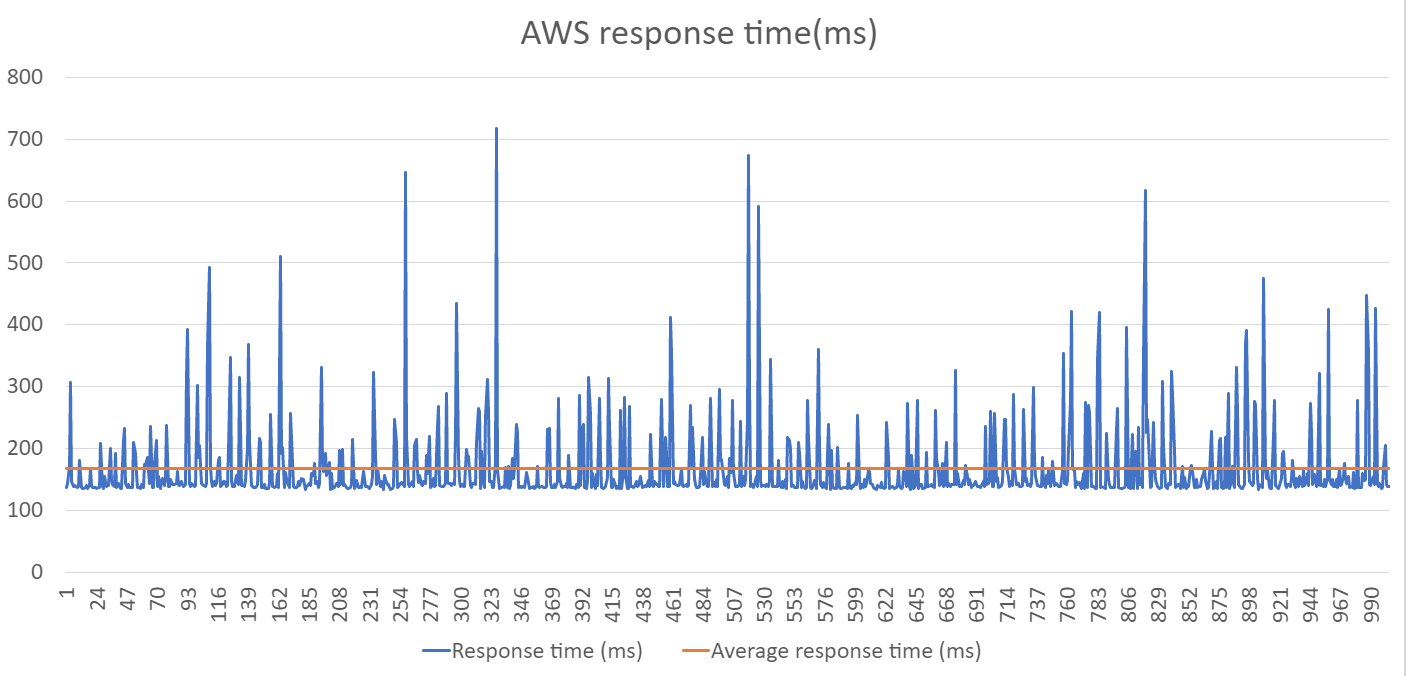
\includegraphics[width=\textwidth]{Pictures/AWS_response_time.png} 
    \caption{Response time and average of AWS}
    \label{AWS response time}
\end{figure}

\begin{figure}[h!]
    \centering
    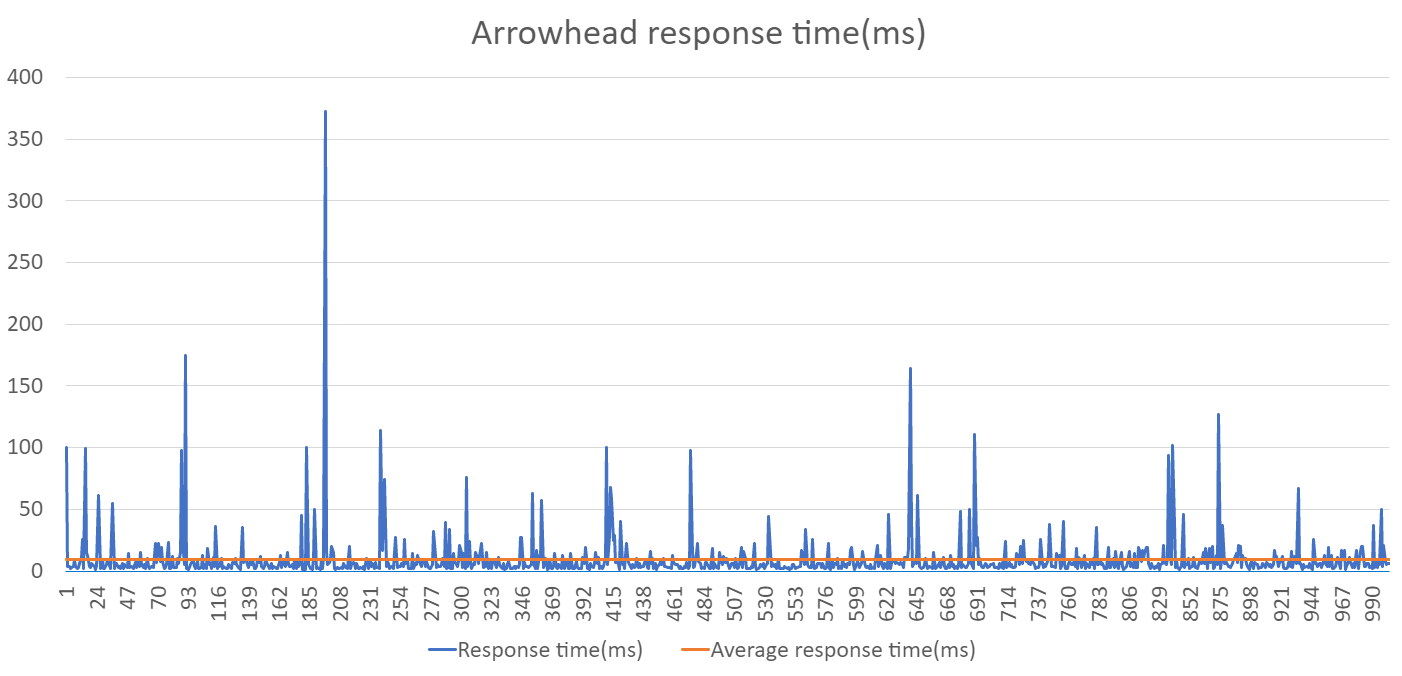
\includegraphics[width=\textwidth]{Pictures/AH_response_time.png} 
    \caption{Response time and average of Arrowhead framework}
    \label{AH response time}
\end{figure}

To give a clearer picture of the results in the test te following table was constructed. 
\begin{center}
    \begin{tabular}{||c|c|c|c||}
        \hline
        Parameters & AWS & Arrowhead \\
        \hline\hline
        Average response time(ms) & 166.94 & 9.5105 \\
        Max response time(ms) & 717 & 372 \\
        Min response time(ms) & 134 & 1 \\
        \hline
    \end{tabular}
\end{center}
The table above shows that the Eclipse Arrowhead framework has the shortest average response time, 17.5 times faster than Amazon Web Services. 
The table also shows that Amazon Web Services has a max response time  1.9 times greater than the Eclipse Arrowhead framework.
We can see the most considerable difference occurs in the minimum response time, where the Eclipse Arrowhead framework is 134 times faster than Amazon Web Services.
The subsequent chapter will cover the advantages of having a quicker response time.


